\chapter{Implementation}
\section{Requirements and Goals}
Depending upon the function we can split the design of a PMU in three parts. 
A. Signal Input \& Sampling part
B. Processing of Samples  
C. Transmission of data
Here different parts will have different requirements. So, we will first state the minimum requirement stated by standards or aimed by us.

\begin{enumerate}
	\item \textbf{ADC Requirements}
	While deciding upon the ADC specification we kept following requirements: 
	\begin{itemize}
		\item Good sampling rate: ~64 Samples/cycle
		\item No of channels: 3 + 3 = 6 (3 - $\phi$ voltage and current) 
		\item Interfacing type: It should be memory addressable and voltage level compatible .
		\item Input type: FSS analog output is differential which can be configured as single ended, it's voltage level is $\pm$10V
	\end{itemize}
	
	\item \textbf{Processing Requirements}
	PMU has stringent timing requirement, samples needs to be processed in given deadline of reporting time, for this a processor having good ALU would be preferable, for which DSP core is best suited for rapid low level and hard realtime computation. Normal Discrete Fourier Transform requires of complexity O($N^{2}$) operations hence the computation requirement increases as the sample count increases. 
	
	\item \textbf{Data Transmission Requirements }
	Realtime transmission of data is mandated by the standards \cite{c37.118}. For that different protocols like Realtime  Media Transfer Protocol (RMTP) or other ways can be used but it would require a sufficiently capable ethernet socket, so we decided to have at least 10/100 MBPs.
	
\end{enumerate}

Initially we decided to use TI OMAPL-137 which is a dual asymmetric-core processor, in which one core is of DSP and other one is of ARMv7 a brief description is given in Appendix. Due to a mishap our OMAP L137 stopped working so new processor was chosen. which was AM3359 which is a single core ARM Cortex-A8, 1 GHz processor, we decided to use BeagleBone Black which is an low-coast open source community supported multipurpose board. All hardware design is made available and complete programmatic access to the hardware is given which gives complete flexibility for development and implementation. Simplified technical description of the board is given below:
\begin{table}[h]
		\begin{center}
			\setlength\arrayrulewidth{1pt}
			\begin{tabular}{|c|c|}
				\hline
				Processor & Sitara AM3358BZC 1 GHz, 2000MIPS\\
				\hline
				Graphic Engine  SGX530 3D, 20M & Polygons/S\\
				\hline
				SDRAM Mem & 512 MB DDR3L 800MHz \\
				\hline
				Onboard Flash 4GB, 8-bit Embedded MMC \\
				\hline
				Serial Port & UART0-4 via 6 pin header 3.3V TTL\\ 
				\hline
				HS USB 2.0 Client ports & USB0 access to client via mini-USB\\
				\hline
				HS USB 2.0 Host Port & Type -A Socket 500mA \\
				\hline
				Ethernet & 10/100, RJ45 \\
				\hline
				SD/MMC Connector & microSD, 3.3 V\\
				\hline
				Video Output & 16b HGMI, 1280x1024 (MAX)\\
				\hline 
				\multirow{3}{10pt}{Expansion Connectors} & power 5v, 3.3V, VDD\_ADC (1.8v) GPIO(69 Pins), LCD, GPMC, MMC1 MMC2 7 ADC in-pins	XDMA Interrupt,
				Power button, Expansion Board ID\\
				\hline
				
			\end{tabular}
		\end{center}
\end{table}

As we can see, specification are pretty impressive but the most important feature of this board are the PRU-ICSS, Programmable Realtime Units Industrial Communication subsystems. Which are two independent 200Mhz 32bit RISC cores . They operate completely independent from the the ARM core,  allowing independent operation and clocking for greater efficiency and flexibility. The PRU-ICSS enables additional peripheral interfaces and real-time protocols. In addition they have fixed execution time, they are connected to (almost) all peripherals with Enhanced Data Bus for (for GPIO for) better communication. PRUs can be programmed separately by loading them with a binary file. Brief description of PRUs are given below

\subsection{PRU Subsystem}
The Programmable Real-Time Unit Subsystem and Industrial Communication Subsystem (PRU-ICSS) consists of dual 32-bit RISC cores (Programmable Real-Time Units, or PRUs), shared, data, and instruction memories, internal peripheral modules, and an interrupt controller (INTC). The programmable nature of the PRU, along with its access to pins, events and all SoC resources, provides flexibility in implementing fast real-time responses, specialized data handling operations, custom peripheral interfaces, and in offloading tasks from the other processor cores of the system-on-chip (SoC).

\begin{figure}
	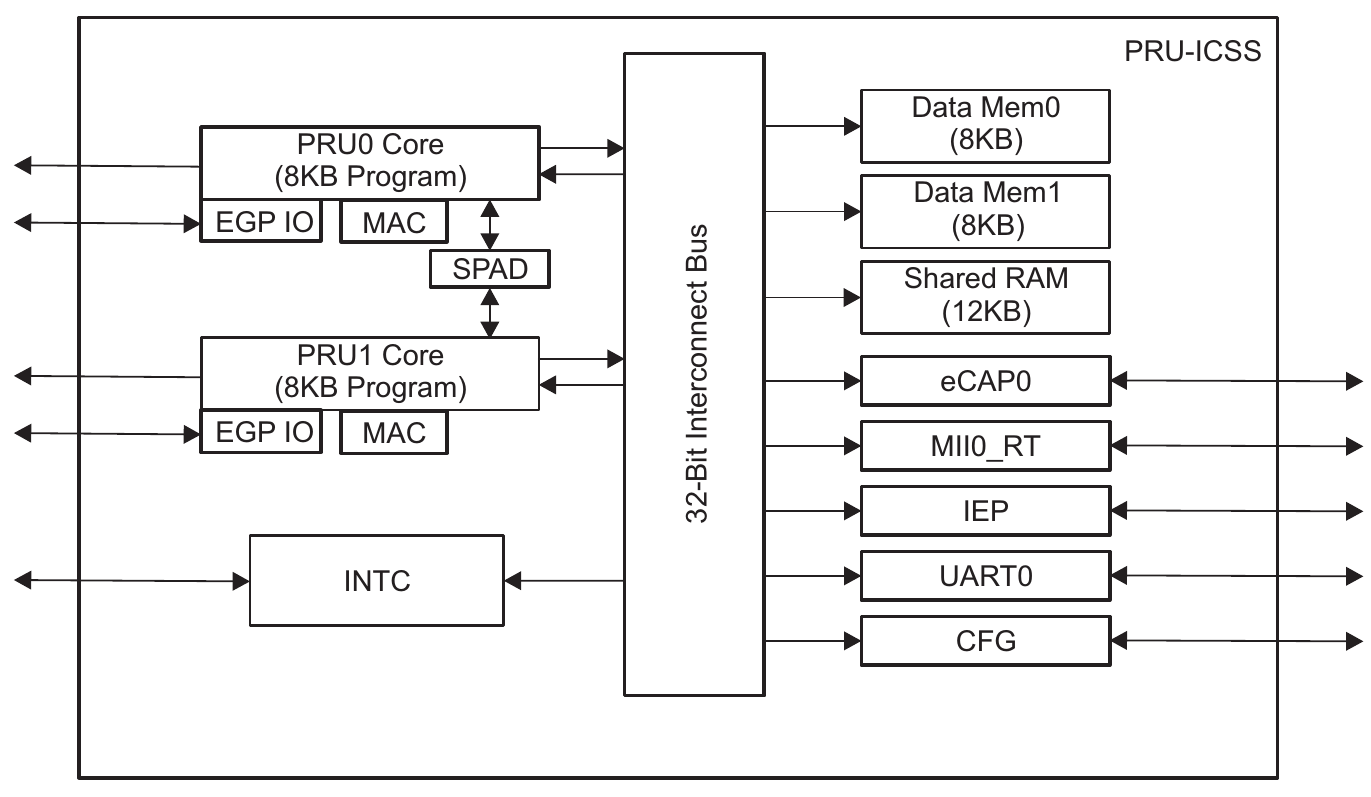
\includegraphics[width=\textwidth]{fig/PRUIcss.png}
	\caption{Block Diagram of PRU Subsystem}
	\label{fig:prublkdrg}
\end{figure}

Useful features that we are using and are worth noting are as follow:
\begin{itemize}
	\item Two PRUs each with:
	\begin{itemize}
		\item 8KB program memory
		\item 8KB data memory
		\item High Performance Interface/OCP Master port for accessing external memories
		\item Enhanced GPIO (EGPIO) with async capture and serial support
		\item Multiplier with optional accumulation (MPY/MAC)		
	\end{itemize}
	\item scratch pad (SPAD) memory with 3 banks of 30, 32-bit registers 
	\item Broadside direct connect between PRU cores within subsystem
	\item 12 KB general purpose shared memory
	\item One Interrupt Controller
	\item One 16550-compatible UART with a dedicated 192-MHz clock.
\end{itemize} 

